%%%%%%%%%%%%%%%%%%%%%%%%%%%%%%%%%%%%%%%%%
% Beamer Presentation
% LaTeX Template
% Version 1.0 (10/11/12)
%
% This template has been downloaded from:
% http://www.LaTeXTemplates.com
%
% License:
% CC BY-NC-SA 3.0 (http://creativecommons.org/licenses/by-nc-sa/3.0/)
%
%%%%%%%%%%%%%%%%%%%%%%%%%%%%%%%%%%%%%%%%%

%----------------------------------------------------------------------------------------
%	PACKAGES AND THEMES
%----------------------------------------------------------------------------------------

\documentclass[t]{beamer}

\mode<presentation> {

% The Beamer class comes with a number of default slide themes
% which change the colors and layouts of slides. Below this is a list
% of all the themes, uncomment each in turn to see what they look like.

%\usetheme{default}
%\usetheme{AnnArbor}
%\usetheme{Antibes}
%\usetheme{Bergen}
%\usetheme{Berkeley}
%\usetheme{Berlin}
%\usetheme{Boadilla}
%\usetheme{CambridgeUS}
%\usetheme{Copenhagen}
%\usetheme{Darmstadt}
%\usetheme{Dresden}
%\usetheme{Frankfurt}
%\usetheme{Goettingen}
%\usetheme{Hannover}
%\usetheme{Ilmenau}
%\usetheme{JuanLesPins}
%\usetheme{Luebeck}
\usetheme{Madrid}
%\usetheme{Malmoe}
%\usetheme{Marburg}
%\usetheme{Montpellier}
%\usetheme{PaloAlto}
%\usetheme{Pittsburgh}
%\usetheme{Rochester}
%\usetheme{Singapore}
%\usetheme{Szeged}
%\usetheme{Warsaw}

% As well as themes, the Beamer class has a number of color themes
% for any slide theme. Uncomment each of these in turn to see how it
% changes the colors of your current slide theme.

%\usecolortheme{albatross}
%\usecolortheme{beaver}
%\usecolortheme{beetle}
%\usecolortheme{crane}
%\usecolortheme{dolphin}
%\usecolortheme{dove}
%\usecolortheme{fly}
%\usecolortheme{lily}
%\usecolortheme{orchid}
%\usecolortheme{rose}
%\usecolortheme{seagull}
%\usecolortheme{seahorse}
%\usecolortheme{whale}
%\usecolortheme{wolverine}

%\setbeamertemplate{footline} % To remove the footer line in all slides uncomment this line
%\setbeamertemplate{footline}[page number] % To replace the footer line in all slides with a simple slide count uncomment this line

%\setbeamertemplate{navigation symbols}{} % To remove the navigation symbols from the bottom of all slides uncomment this line
}

\usepackage{graphicx} % Allows including images
\usepackage{booktabs} % Allows the use of \toprule, \midrule and \bottomrule in tables
\usepackage[normalem]{ulem}

%----------------------------------------------------------------------------------------
%	TITLE PAGE
%----------------------------------------------------------------------------------------

\title[]{Breadboard to Printed Circuit Board} % The short title appears at the bottom of every slide, the full title is only on the title page

\author{Josh Johnson} % Your name
\institute[] % Your institution as it will appear on the bottom of every slide, may be shorthand to save space
{ \\ % Your institution for the title page
\medskip
\textit{} % Your email address
}
\date{10/6/2019} % Date, can be changed to a custom date

\begin{document}

\begin{frame}
\titlepage % Print the title page as the first slide
\end{frame}

%----------------------------------------------------------------------------------------
%	PRESENTATION SLIDES
%----------------------------------------------------------------------------------------


\begin{frame}
\frametitle{Motivation}
\begin{itemize}
	\item So you have a circuit working on a breadboard, however you need to move it to a PCB.
	\item You might also have an idea for a design which can't be breadboarded, and want your PCB work the first time.
	\item You might need it to be battery powered, have a certain form factor, or be lower cost.
	\item Maybe you are producing them in quantity, or are taking the level of integration up a notch.
\end{itemize}
\vspace{3mm}
How can you achieve these goals? 



\vspace{15mm}
Project Files: \url{github.com/joshajohnson/CBRhardware}\\
\end{frame}

%----------------------------------------------------------------------------------------

\begin{frame}[t]
\frametitle{Key Considerations}

\begin{itemize}
	\item What quantity is being produced?
	\item How much time do I have to spend on the project?
	\item What size / type of components am I willing to work with?
	\item I have an development / breakout board, how do I replace it with discrete parts?
	\item How am I going to program it?
	\item How will I communicate with it?
	\item How do I want to power it?
	\item \sout{How will Josh debug it when he makes mistakes?} 
	\item Mechanical design considerations. 
\end{itemize}

\end{frame}

%----------------------------------------------------------------------------------------

\begin{frame}
\frametitle{Key Considerations}
\large{\textbf{What quantity is being produced?}}
\vspace{1mm}
\begin{itemize}
	\item Low volume 
	\begin{itemize}
		\item Trade off complexity for cost. Examples are prebuilt modules, commonly used parts, flying wires.
	\end{itemize} 
	\item Medium volume
	\begin{itemize}
		\item Cost starts to become a consideration. See if a small amount of R\&D can lower the bill of materials.
		\item Assembly time - small changes (single sided load, surface mount parts) multiply out to save a lot of time.
	\end{itemize}
	\item Large volume
	\begin{itemize}
		\item I'm not qualified to talk to this, but more time can be spent in R\&D if it means lower BOM and assembly. e.g. Capacitative buttons vs mechanical, code optimisation vs larger microprocessor. 
	\end{itemize}
\end{itemize}
\end{frame}

%----------------------------------------------------------------------------------------

\begin{frame}
\frametitle{Key Considerations}
\large{\textbf{How much time to I have to spend on the project?}}
\vspace{1mm}

\begin{itemize}
	\item Similar considerations to quantity, if short on time, look for more integrated solutions. 
	\begin{itemize}
		\item Display on PCB with 0.1" headers vs display + supporting passives.  
		\item Arduino Nano / Pro Mini vs DIY ATmega 328p.
		\item Power supply brick / LIPO charge module vs rolling your own. 
		\item Steal designs from Adafruit / Sparkfun. 
	\end{itemize}
\end{itemize}
\end{frame}

%----------------------------------------------------------------------------------------

\begin{frame}
\frametitle{Key Considerations}
\large{\textbf{What size / type of components am I willing to work with?}}
\vspace{1mm}
\begin{itemize}
	\item Through hole vs surface mount
	\begin{itemize}
		\item With correct tools, SMT is quicker and easier than THT. 
		\item THT is easier to resolve bugs, but takes up more space and some parts are SMT only. 
	\end{itemize} 
	\item Component size
	\begin{itemize}
		\item What sizes are parts available in? e.g. DIP vs SOIC vs TQFP vs QFN.
		\item Who is assembling them? e.g. if first timers, go with easier parts. 
		\item With time, you will figure out what size parts you are happy working with. I personally suggest 0603 if you have steady hands / good eyesight, 0805/1206 otherwise, but larger parts are harder to source. 
	\end{itemize}
	\item Space constraints
	\begin{itemize}
		\item Do you have to use small parts due to form factor / performance reasons? e.g. 0402 result in less impedance mismatch on traces, however you can use 0603 decoupling caps with little downside.   
	\end{itemize}
\end{itemize}
\end{frame}

%----------------------------------------------------------------------------------------

\begin{frame}
\frametitle{Key Considerations}
\large{\textbf{I have an development / breakout board, how do I replace it with discrete parts?}}
\vspace{1mm}
\begin{itemize}
	\item Reference designs 
	\begin{itemize}
		\item Find who makes the board you are using and look for a schematic.
		\item If unmarked, probably a Sparkfun / Adafruit clone - look on their website.
	\end{itemize} 
	\item Datasheet / application notes
	\begin{itemize}
		\item Google is your friend.
		\item Datasheets typically have a recommended schematic 1/3 down. 
		\item Application notes go into more detail regarding function of the device and different configurations. 
		\item Manufacturer probably has an evaluation board with schematics available.
	\end{itemize}
	\item Substitutions
	\begin{itemize}
		\item Many parts can be substituted for a similar component. e.g. mosfets, transistors, voltage regulators. 
		\item If looking for a substitute, Texas Instruments, and Analog Devices have great datasheets and app notes. 
	\end{itemize}
\end{itemize}
\end{frame}

%----------------------------------------------------------------------------------------

\begin{frame}
\frametitle{Key Considerations}
\large{\textbf{How am I going to program it?}}
\vspace{1mm}
\begin{itemize}
	\item Does my device have a bootloader?
	\begin{itemize}
		\item 'Arduino compatible' devices all have bootloaders which new ICs don't. 
		\item Flashing bootloaders may require UART, SPI, SWD, JTAG depending on chip, may also require dedicated programming header.  
	\end{itemize} 
	\item UART / Serial
	\begin{itemize}
		\item Many ICs will have a DFU pin which if held low on startup, will load code from a serial port. 
		\item STM32, ESP8266 / ESP32, my reflow oven (freescale?), many others are examples of this.
	\end{itemize}
	\item Serial  Peripheral Interface
	\begin{itemize}
		\item ATmega / ATtiny microprocessors are flashed via SPI.
		\item Programmer also required to set fuse bits.   
	\end{itemize}
	\item Single Wire Debug
	\begin{itemize}
		\item ARM Cortex cores - two pins + power allow programming and debugging. 
	\end{itemize}
\end{itemize}
\end{frame}

%----------------------------------------------------------------------------------------

 \begin{frame}
 \frametitle{Key Considerations}
 \large{\textbf{ How will I communicate with it?}}
 \vspace{1mm}
 \begin{itemize}
 	\item Serial
 	\begin{itemize} 
 		\item Serial is the easiest method, but will require USB <-> Serial converter. 
 		\item Can place converter on board with USB connector, or leave header exposed and use dedicated cable.
 		\item Flashing with a serial bootloader is common, e.g. Arduino series. 
 		\item May require reset circuit for serial programming with bootloader. 
 	\end{itemize} 
 	\item USB
 	\begin{itemize}
 		\item USB bootloaders allow for updating over a USB cable, no other parts required. 
 		\item If you device has native USB, setting it up as a virtual COM port makes computer think it is a serial port. 
 		\item Can also do HID emulation to pretend to be a keyboard/mouse. 
 	\end{itemize}
 	\item Wireless
 	\begin{itemize}
 		\item Wireless communications / firmware updating is possible, serial over bluetooth is common for communications. 
 	\end{itemize}
 \end{itemize}
\end{frame}

%----------------------------------------------------------------------------------------

\begin{frame}
\frametitle{Key Considerations}
\large{\textbf{ How will I power it?}}
\vspace{1mm}
\begin{itemize}
	\item Power supply methods
	\begin{itemize}
		\item USB (5V)
		\item Battery (Coin Cell, AA, LIPO)
		\item 9/12 VDC
	\end{itemize}
	\item Voltage regulation
	\begin{itemize}
		\item Low current OR small input -> output difference: linear regulator.
		\item High current OR large input -> output difference OR output > input: switchmode supply.
	\end{itemize}
	\item Rechargeable batteries.
	\begin{itemize}
		\item Ensure each cell has charge protection built in.
		\item Use a charge controller IC.
		\item If using LIPO with circuit at 3V3, can get away with a linear regulator.
		\item If 5V is required, boost converter will need be used.
		\item Can connect directly to battery as well e.g. Neopixel VCC. 
	\end{itemize}
\end{itemize}
\end{frame}

%----------------------------------------------------------------------------------------

\begin{frame}
\frametitle{Key Considerations}
\large{\textbf{How will I debug it?}}
\vspace{1mm}
\begin{itemize}
	\item Power
	\begin{itemize}
		\item Status LEDs on power rails.
		\item Using 1V8? Low Vgs N channel Mosfet on low side of LED. 
		\item Test points (and ground pads) for every voltage rail.
		\item Allow board to be powered from a bench supply, through Vin connection.
	\end{itemize}
	\item Microcontroller
	\begin{itemize}
		\item If using a microcontroller / toolchain with debug support, have a debug header on the board. 
		\item Serial (UART) comms are great to have broken out, even if using USB. 
	\end{itemize}
	\item On Board signals
	\begin{itemize}
		\item Test points, test points, test points.
		\item 1 mm diameter SMD pads don't take up much room, can be easily soldered onto. 
		\item SMD test points (metal loops) are a great option for ground. 
		\item Test points are less useful without plenty of available grounds.
	\end{itemize}
\end{itemize}
\end{frame}

%----------------------------------------------------------------------------------------

\begin{frame}
\frametitle{Key Considerations}
\large{\textbf{Mechanical Considerations}}
\vspace{1mm}
\begin{itemize}
	\item Board size / shape
	\begin{itemize}
		\item Does the board need to fit into a pre defined area?
		\item Do components (connectors, displays, buttons, LEDs) need to be located in a certain position or on a certain side?
	\end{itemize}
	\item Enclosure choice
	\begin{itemize}
		\item Does my board need an enclosure?
		\item If so, do I want to make my own or purchase a prebuilt enclosure?
		\item Plastic box vs aluminium extrusion vs acrylic vs 3D printed. 
	\end{itemize}
	\item Mechanical Modelling 
	\begin{itemize}
		\item Import .STEP into ECAD as a 3D model for a footprint.
		\item Export .STEP from ECAD into MCAD (I use KiCad and Fusion360).
		\item Draw enclosure around board OR check board fits in designed enclosure.
		\item Can export .DXF from MCAD into ECAD, and design board around that. 
	\end{itemize}
\end{itemize}
\end{frame}

%----------------------------------------------------------------------------------------

\begin{frame}[t]
\frametitle{Snapchat Glasses}
\begin{figure}
	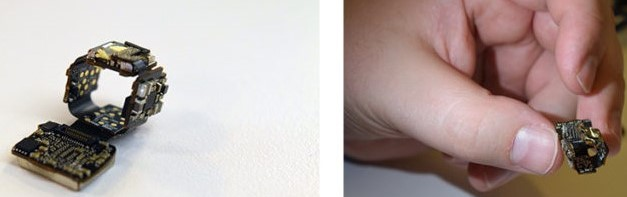
\includegraphics[width=\linewidth]{snapGlasses.jpg}
\end{figure}
\begin{figure}
	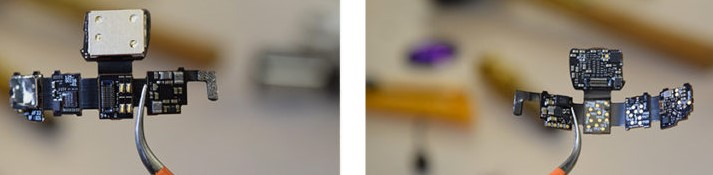
\includegraphics[width=\linewidth]{snapGlasses2.jpg}
\end{figure}

\end{frame}
%----------------------------------------------------------------------------------------

\begin{frame}[t]
\frametitle{Casper Night Light}
\begin{figure}
	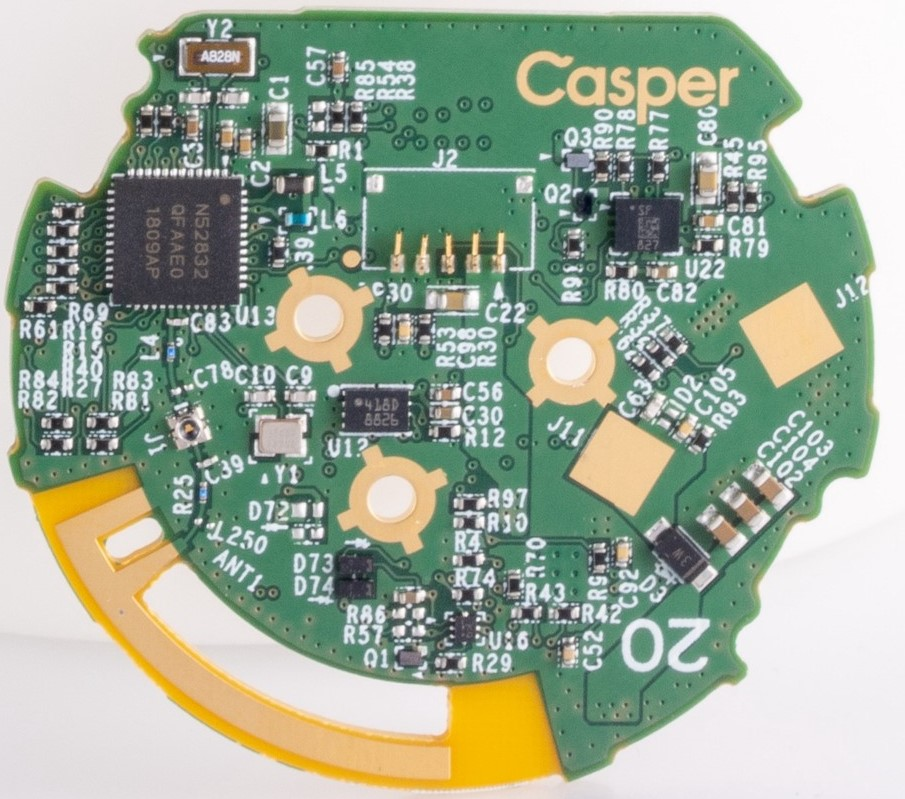
\includegraphics[width=0.7\linewidth]{casper.jpeg}
\end{figure}
\end{frame}
%----------------------------------------------------------------------------------------

\begin{frame}[t]
\frametitle{Casper Night Light}
\begin{figure}
	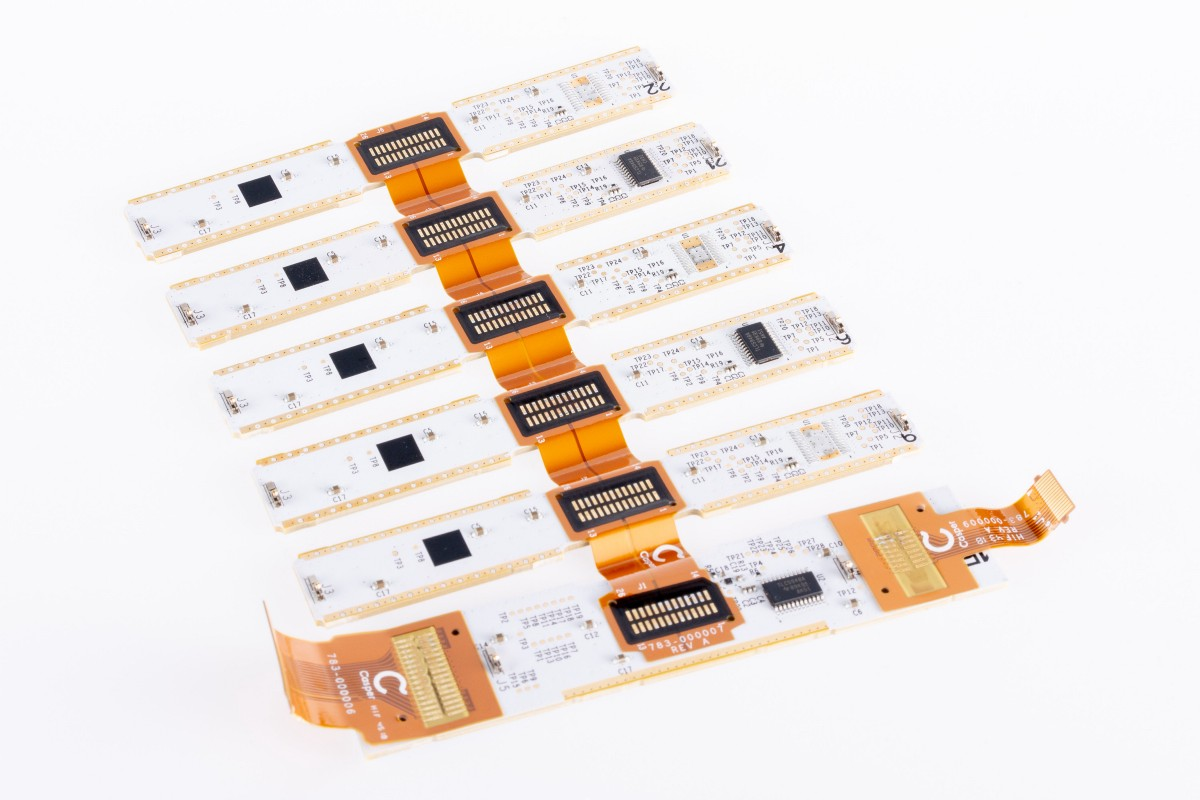
\includegraphics[height=0.75\textheight]{casper2.jpeg}
\end{figure}

\end{frame}
%----------------------------------------------------------------------------------------


\begin{frame}
\frametitle{</talk>}

Say Hello! \\
BSidesCbr Slack: josh\\
Twitter: @\textunderscore joshajohnson\\
Email: josh@joshajohnson.com\\
\vspace{4mm}

Project Files: \url{github.com/joshajohnson/CBRhardware}\\
\end{frame}


\end{document} 